\section{Introduction}
The Demo Description Lines (DDL) define an abstract syntax, written in JSON (JavaScript Object Notation) format, that specifies the IPOL demos. Their main objective is to simplify as much as possible the creation of demos by describing them without the need of writing Python or HTML. This allows fast demo editing in the journal. The following sections describe each of the main keys of the DDL:

\begin{itemize}
  \item \textit{general}: general options (required);
  \item \textit{build}: download and compile the source code (required);
  \item \textit{inputs}: description of the inputs  (optional);
  \item \textit{params}: description of the parameters and user control (optional);
  \item \textit{run}: script or binary which needs to be called for the execution, along with its parameters (required);
  \item \textit{archive}: which parameters and files will be stored in the archive (optional);
  \item \textit{results}: which elements will be displayed as results (required).
\end{itemize}

\vspace{1em}

The IPOL control panel provides a JSON editor with a simple validator. Most of the syntax errors are detected in real time and reported by this graphical tool.

%-------------------------------------------------------------------------------
\section{The \emph{general} section}
The general section describes global information about the demo. It is a set of (key, value) pairs, described in the following table. The column \emph{req} refers to a required field. This type of tables will be used in all the sections of this document.

% 
\begin{longtable}{|>{\bf}L{\dimexpr 0.28\linewidth}|L{\dimexpr 
0.57\linewidth}|c|}
\hline
 \centering {key}     & \centering {\bf description} & {\bf req} 
\tabularnewline \hline \hline
 demo\_title         & Title of the demo. & no\\ \hline
 input\_description  & Description of the inputs. It contains HTML as a single string or as an array of string that will be concatenated and separated with spaces. & no \\ \hline
 param\_description  & Description for the parameters. It contains HTML code as a single string or as an array of string that will be concatenated and separated with spaces. & no
\\ \hline
 xlink\_article     & Link to the article webpage & no  \\ \hline
 requirements 	    & It specifies particular requirements needed for the execution of the demo, separated by commas. e.g. Matlab. & no \\ \hline
 timeout 	    & It specifies maximum time in seconds allows to execute the algorithm. If the execution takes longer than the specified time the system stops the exection. & no \\ \hline
\caption{Fields in the \emph{general} section.}
\end{longtable}

%-------------------------------------------------------------------------------
\section{The \emph{build} section}

The build section is a set of one or more sets, each one providing information to obtain and compile the source codes needed for a given demo. If the demo needs to compile several files from different links, the build sets must be indexed as build1, build2,..., build\textit{n} being \textit{n} the total number of builds (see the example below). It is mandatory to write at least build1. Three steps are needed to build a demo: 

\begin{itemize}
  \item Download the original sources codes (with optional userid and password for private demos);
  \item Build the executables after the download;
  \item Copy the needed files in a run context to execute the  demo.
\end{itemize}

\begin{longtable}{|>{\bf}L{\dimexpr 0.25\linewidth}|L{\dimexpr 0.6\linewidth}|c|}
\hline
\centering {key}     & \centering {\bf description} & {\bf req} \tabularnewline 
\hline \hline
 url        & Link to download the source codes as a compressed file. & yes \\ \hline
 username   & Username for private demos. & no \\ \hline
 password   & Password for private demos. & no \\ \hline
 construct  & Shell command needed to compile the downloaded source code. & no  \\ \hline
 move       & List of files needed to execute the demo separated with commas (see example below) & yes  \\ \hline
\caption{Build fields}
\end{longtable}

\paragraph{Example:}
In this case, the demo needs to compile from two different compressed files. The DDL uses the \textit{move} statement to copy the obtained files after the compilation into a run context.%\\
\begin{lstlisting}[language=json,firstnumber=1]
"build": {
    "build1": {
        "url": "http://www.ipol.im/pub/art/2014/82/sift_anatomy_20141201.zip",
        "construct": "cd sift_anatomy_20141201 && make",
        "move": "sift_anatomy_20141201/bin/sift_cli, sift_anatomy_20141201/bin/match_cli"
    },
    "build2":{
        "url": "http://dev.ipol.im/~monasse/orthoPose_1.0.tar.gz",
        "construct": "matlab -nodisplay -nosplash -nodesktop -r \"cd orthoPose_1.0/; mcc -m mainPoseEstimation.m -a lib/; exit;\"",
        "move": "orthoPose_1.0/mainPoseEstimation, orthoPose_1.0/run_mainPoseEstimation.sh"
    }
}
\end{lstlisting}

%-------------------------------------------------------------------------------
\section{The \emph{inputs} section}
The inputs section describes the characteristics of the input data for the algorithm.

\subsection{The \emph{image} type}

\begin{longtable}{|>{\bf}L{\dimexpr 0.26\linewidth}|L{\dimexpr 0.59\linewidth}|c|}
\hline
\centering {key}     & \centering {\bf description} & {\bf req} \tabularnewline 
\hline \hline
 type         & type of the input: image & yes \\ \hline
 description  & Short name or description. This is used by the web interface. & no \\ \hline
 max\_pixels  & This value sets the maximum number of pixels allowed for the input. If the size of the image is over this the limit it will be resized. The value can be a number or an arithmetic expression (ex:  ``1000*1000" = 1 Mpx).  & yes \\ \hline
 max\_weight   & Maximum weight (in bytes) of an input file. This prevents uploading too large files. The value can be a number or an arithmetic expression (ex: ``100*1024*1024"= 100 Mb). & no \\ \hline
 dtype        & Final format for the image. Some examples:
\begin{itemize}
  \setlength\itemsep{-0.5em}
  \item \textit{1x8i}: gray, unsigned integer 8 bits;
  \item \textit{3x8i}: color, RGB unsigned integer 8 bits;
  \item \textit{1x16i}: gray, unsigned integer 16 bits;
  \item \textit{3x16i}: color, RGB unsigned integer 16 bits.
\end{itemize} 
 & yes \\ \hline
 ext          & input extension (ie. file format) & yes \\ \hline
forbid\_preprocess & Forbids any pre-processing of the input data. 
Submitted image is kept as-is. Used by algorithms like noise estimation or modification detection, where re-sampling will affect results. 
If a processing is needed according to the expected properties, an error message will be displayed to the user.
& no \\ \hline
\caption{Fields for an \emph{image} as input.}
\end{longtable}

\subsection{The \emph{video} type}

\begin{longtable}{|>{\bf}L{\dimexpr 0.26\linewidth}|L{\dimexpr 0.59\linewidth}|c|}
\hline
\centering {key}     & \centering {\bf description} & {\bf req} \tabularnewline 
\hline \hline
 type         & type of the input: video & yes \\ \hline
 description  & Short name or description. This is used by the web interface. & no \\ \hline
 as\_frames & Boolean value. The input video will be converted to png images for each frame according to the max\_frames field. Frames
 will be stored in a temporal folder inside the execution directory with the name. (ex: ./input\_0/frame\_000.png ) & no \\ \hline
 max\_pixels   & This value sets the maximum number of pixels allowed for the input video per frame. If the size of the input is over, the video frames will be resized. The value can be a number or an arithmetic expression (ex: ``1000*1000" = 1 Mpx).  & yes \\ \hline 
 max\_frames  &  Maximum number of frames after conversion, either as frames or video.  & yes \\ \hline
 max\_weight   & Maximum weight (in bytes) of an input file. This prevents uploading too large files. The value can be a number or an arithmetic expression (ex: ``100*1024*1024"= 100 Mb). & no \\ \hline
forbid\_preprocess & Forbids any pre-processing of the input data by the IPOL system. Submitted video is kept as-is. Used by algorithms like noise-estimation or modification detection, where re-sampling will affect results.If a processing is needed according to the expected properties, an error message will be displayed to the user.
& no \\ \hline
\caption{Fields for a \emph{video} as input.}
\end{longtable}

%-------------------------------------------------------------------------------
\section{The \emph{params} section}
The \emph{params} section describes the set of parameters needed by a demo, their constraints and the visual appearance of the user control. It is defined as an array of sets, where each set contains (key, value) pairs. In this section, we show examples of the expected appearance of these parameters in the web interface. The look of the controls might differ depending on the operating system and the browser used.

\subsection{The \emph{range} type}

The \emph{range} type is used as an horizontal slider constrained by a minimum and a maximum numeric values. It can be moved with the mouse or by using the arrow keys according to the step value fixed in the DDL. The user control is similar to the one at figure~\ref{fig:sliders}.

\begin{longtable}{|>{\bf}L{\dimexpr 0.15\linewidth}|L{\dimexpr 
0.7\linewidth}|c|}
\hline
 \centering {key}     & \centering {\bf description} & {\bf req} 
\tabularnewline \hline \hline
 type   & range       & yes \\ \hline
 id     & Used to identify the parameter. & yes \\ \hline
 label  & A name and/or description of the parameter. It appears on the left side in the web interface. & no
                      \\ \hline
 comments & A description of the parameter. It appears on the right side in the web interface. & no
                      \\ \hline
 visible    & Javascript expression evaluated as a boolean. & no \\ \hline
 values & Sets min, max, step and default values using a key/value 
scheme \{ 'min':val, 'max':val, 'step':val, 'default':val \}. 
Ex: to select a value included in (-1, -0.5, 0, 0.5, 1) write \texttt{"values": \{"min": -5, "max": 5, "step": 0.5, "default": 0\}}  & yes
                      \\ \hline
\caption{Fields for the properties of the \emph{range} type.}
\end{longtable}

\begin{figure}[h]
\centering
\tcbox[sharp corners, boxsep=0.0mm, boxrule=0.5mm, colback=white]{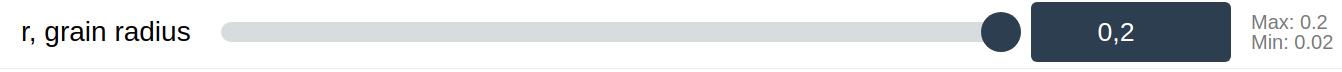
\includegraphics[scale=0.35]{Images/slider_examples.png}}
\caption{Range type example. It shows a slider with values from 0.02 to 0.2.}
\label{fig:sliders}
\end{figure}

\subsection{The \emph{selection\_collapsed} type}

The \emph{selection\_collapsed} type returns one string selected by a key (for example, a color code selected by name). The user control is a dropdown select similar to the one in figure~\ref{fig:selection_collapsed_example}.

\begin{longtable}{|>{\bf}L{\dimexpr 0.25\linewidth}|L{\dimexpr 
0.6\linewidth}|c|}
\hline
 \centering {key}     & \centering {\bf description} & {\bf req} 
\tabularnewline \hline \hline
 type  & selection\_collapsed    & yes \\ \hline
 id     & Used to identify the parameter. & yes \\ \hline
 label  & A name and/or description of the parameter. It appears on the left side in the web interface. & no
                      \\ \hline
 comments & A description of the parameter. It appears on the right side in the web interface. & no
                      \\ \hline
 visible    & Javascript expression evaluated as a boolean.
            & no \\ \hline
 values & set of (key, value) pairs, where the key is the displayed text and the 
value is the string returned, for example \texttt{"values": \{"black": "000000", "white": "FFFFFF"\}} & yes
                      \\ \hline
 default\_value & defines the default value for this parameter, should be one 
the values defined in 'values'. & yes \\ \hline
\caption{Fields for the properties of the \emph{selection\_collapsed} type.}
\end{longtable}

\begin{figure}[h]
\centering
\tcbox[sharp corners, boxsep=0.0mm, boxrule=0.5mm, colback=white]{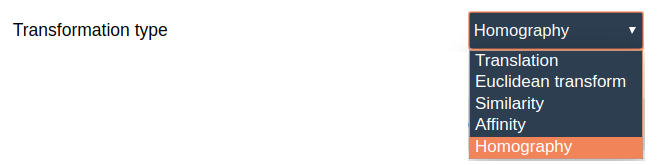
\includegraphics[scale=0.35]{Images/selection_collapsed_example.png}}
\caption{Selection collapsed example. In this case, the selection offers five options to choose.}
\label{fig:selection_collapsed_example}
\end{figure}

\clearpage
\subsection{The \emph{selection\_radio} type}

The \emph{selection\_radio} returns one string selected by a key (for example, a color code selected by name). The user control is a set of radio buttons as in figure~\ref{fig:selection_radio_example}.

\begin{longtable}{|>{\bf}L{\dimexpr 0.25\linewidth}|L{\dimexpr 
0.6\linewidth}|c|}
\hline
 \centering {key}     & \centering {\bf description} & {\bf req} 
\tabularnewline \hline \hline
 type     & selection\_radio    & yes \\ \hline
 id     & Used to identify the parameter. & yes \\ \hline
 label  & Name and/or description of the parameter. It appears on the left side in the web interface. & no
                      \\ \hline
 comments & Description of the parameter. It appears on the right side in the web interface. & no
                      \\ \hline
 visible    & Javascript expression evaluated as a boolean.
            & no \\ \hline
 values   & set of (key, value) pairs, where the key is the displayed text and the 
value is the string returned, for example \texttt{"values": \{"black": "000000", "white": "FFFFFF"\}} & yes
                      \\ \hline
 default\_value & defines the default value for this parameter, should be one 
the values defined in 'values'. & yes \\ \hline
 vertical & It is boolean value. The button distribution is vertical when the value is activated (true), otherwise, the visualization is horizontal as default. & no \\ \hline
\caption{Fields for the properties of the \emph{selection\_radio} type.}
\end{longtable}

\begin{figure}[h]
\centering
\tcbox[sharp corners, boxsep=0.0mm, boxrule=0.5mm, colback=white]{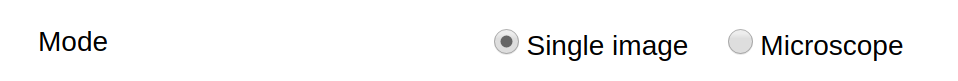
\includegraphics[scale=0.35]{Images/selection_radio_example.png}}
\caption{Radio buttons example. The label description is Mode and the parameter offers two radio buttons. The vertical option is disabled.}
\label{fig:selection_radio_example}
\end{figure}

\subsection{The \emph{label} type}

The \emph{label} type can be used to separate groups of parameters or to include html fields (images, external links, etc.) in the web interface.

\begin{longtable}{|>{\bf}L{\dimexpr 0.27\linewidth}|L{\dimexpr 
0.58\linewidth}|c|}
\hline
 \centering {key}     & \centering {\bf description} & {\bf req} 
\tabularnewline \hline \hline
 type  & label       & yes \\ \hline
 label & HTML text to display, as a single string or as an array of strings. & yes \\ \hline
 visible    & Javascript expression evaluated as a boolean.
            & no \\ \hline
\caption{Fields for the properties of the \emph{label} type.}
\end{longtable}

\begin{figure}[h]
\centering
\tcbox[sharp corners, boxsep=0.0mm, boxrule=0.5mm, colback=white]{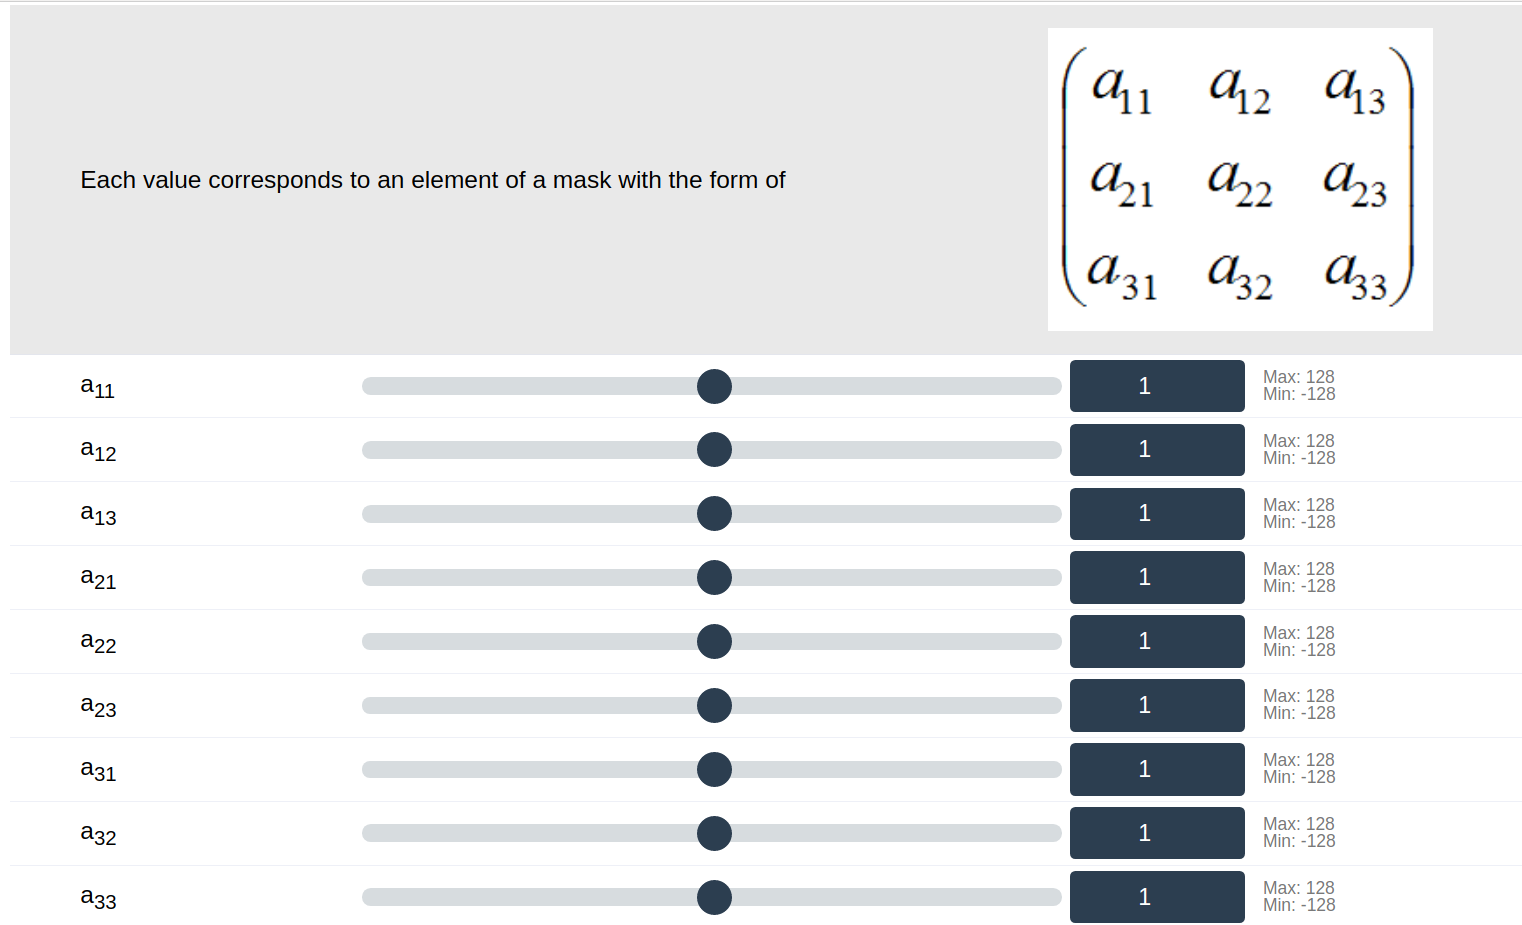
\includegraphics[scale=0.30]{Images/label_example.png}}
\caption{Label example. The label explains that the sliders below represent matrix values according to the image depicted in the label.}
\label{fig:label_example}
\end{figure}

\subsection{The \emph{checkbox} type}

The \emph{checkbox} type returns a boolean value. The user control is a checkbox similar to the one in figure~\ref{fig:checkbox_example}.

\begin{longtable}{|>{\bf}L{\dimexpr 0.27\linewidth}|L{\dimexpr 
0.58\linewidth}|c|}
\hline
 \centering {key}     & \centering {\bf description} & {\bf req} 
\tabularnewline \hline \hline
 type  & checkbox  & yes \\ \hline
 id     & Used to identify the parameter. & yes \\ \hline
 label  & A name and/or description of the parameter. It appears on the left side. & no
                      \\ \hline
 comments & A description of the parameter. It appears on the right side in the web interface. & no
                      \\ \hline
 visible    & Javascript expression evaluated as a boolean. & no \\ \hline
 default\_value & boolean: True for checked & \\ \hline
\caption{Fields that manages the properties of the \emph{checkbox} type.}
\end{longtable}

\begin{figure}[h]
\centering
\tcbox[sharp corners, boxsep=0.0mm, boxrule=0.5mm, colback=white]{
\includegraphics[scale=0.35]{Images/checkbox_example.png}}
\caption{Checkbox example. This can be used in the demos that need to activate or not an option.}
\label{fig:checkbox_example}
\end{figure}

\subsection{The \emph{numeric} type}

The \emph{numeric} type returns a numeric value validated against constraints (min, max). The user control is an input field with numbers. Note that this is quite similar to the \emph{range} type but without the slider. You can see an example in figure~\ref{fig:numeric_example}.

\begin{longtable}{|>{\bf}L{\dimexpr 0.27\linewidth}|L{\dimexpr 
0.58\linewidth}|c|}
\hline
 \centering {key}     & \centering {\bf description} & {\bf req} 
\tabularnewline \hline \hline
 type       & numeric   & yes \\ \hline
 id     & Used to identify the parameter. & yes \\ \hline
 label  & A name and/or description of the parameter. It appears on the left side. & no
                      \\ \hline
 comments & A description of the parameter. It appears on the right side in the web interface. & no
                      \\ \hline
 visible    & Javascript expression evaluated as a boolean. & no \\ \hline
 values     & Set min, max, and default values using the following key/value scheme \texttt{"values": \{"min": -5, "max": 5, "default": 0\}} & yes \\ \hline
\caption{Fields for the properties of the \emph{numeric} type.}
\end{longtable}

\begin{figure}[h!]
\centering
\tcbox[sharp corners, boxsep=0.0mm, boxrule=0.5mm, colback=white]{
\includegraphics[scale=0.30]{Images/numeric_example.png}}
\caption{Numeric example. The label explains that the sliders below represent matrix values according to the image depicted in the label.}
\label{fig:numeric_example}
\end{figure}

\subsection{The \emph{text} type}

The \emph{text} type returns a string. The user control is an input field.

\begin{longtable}{|>{\bf}L{\dimexpr 0.27\linewidth}|L{\dimexpr 
0.58\linewidth}|c|}
\hline
 \centering {key}     & \centering {\bf description} & {\bf req} 
\tabularnewline \hline \hline
 type       & text   & yes \\ \hline
 id     & Used to identify the parameter. & yes \\ \hline
 label  & A name and/or description of the parameter. It appears on the left side. & no
                      \\ \hline
 comments & A description of the parameter. It appears on the right side in the web interface. & no
                      \\ \hline
 visible    & Javascript expression evaluated as a boolean. & no \\ \hline
 values     & set maxlength in characters and default values using the following key/value scheme \texttt{"values": \{"maxlength": 3, "default": "fr"\}} & no \\ \hline
\caption{Fields for the properties of the \emph{text} type.}
\end{longtable}

\begin{figure}[h]
\centering
\tcbox[sharp corners, boxsep=0.0mm, boxrule=0.5mm, colback=white]{
\includegraphics[scale=0.35]{Images/text_example.png}}
\caption{Text example. The user can write some text as parameter for the demo.}
\label{fig:text_example}
\end{figure}


\subsection{The \emph{textarea} type}

This param allows including textual information as a parameter. The text must be written in the DDL with the correct format. This means that the text area can show your message with new lines, skip lines and the normal ways of a file if the encoding format is correct. For instance, if you want that your text area looks like in figure~\ref{fig:textarea_example}, the default value must be as in the following example:

\paragraph{Examples:}
\label{textarea_example}
Example of a DDL when using a text area. %\\
\begin{lstlisting}[language=json,firstnumber=1]
{
  "default_value": "INFORMATION ABOUT FIRST RECTANGLE CONTAINER\r\nNORMALIZED IMAGE DIMENSION\r\nwidth_float = 1.413793\r\n",
            "wrap":false,
            "height": 5,
            "type": "textarea",
            "id": "file_1",
            "label": "Parameter file of the model.",
            "comments":"<b>You can also change the parameters in the text.<b>",
}
\end{lstlisting}


\begin{longtable}{|>{\bf}L{\dimexpr 0.27\linewidth}|L{\dimexpr 
0.58\linewidth}|c|}
\hline
 \centering {key}     & \centering {\bf description} & {\bf req} 
\tabularnewline \hline \hline
 type           & textarea   & yes \\ \hline
 label          & name and/or description of the parameter. It appears on the left side. & no \\ \hline
 id             & Used to identify the parameter. & yes \\ \hline
 default\_value  & Text to include in the text area & no \\ \hline
visible    & Javascript expression evaluated as a boolean. & no  \\\hline
height  & Set the height of your textarea. The maximum value is 2000px.  & no \\ \hline
width  & Set the width of your textarea. If you do not include the parameter it will be 100\%.  & no \\ \hline
wrap   & This attribute specifies how the text in a text area is wrapped. False means that the line is not adapted to the textarea. True the opposite. & no \\ \hline
\caption{Fields for the properties of the \emph{textarea} type.}
\end{longtable}

\begin{figure}[h!]
\centering
\tcbox[sharp corners, boxsep=0.0mm, boxrule=0.5mm, colback=white]{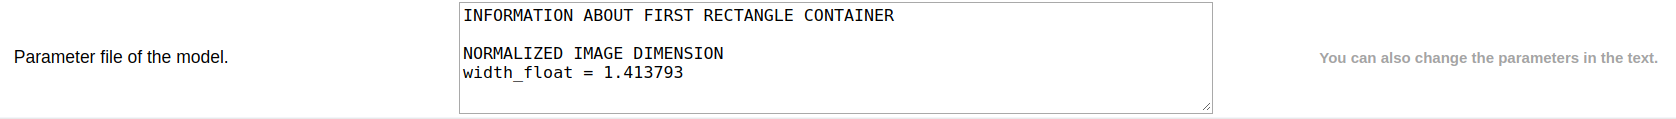
\includegraphics[scale=0.30]{Images/textarea_example.png}}
\caption{textarea example. The label explains that the sliders below represent matrix values according to the image depicted in the label.}
\label{fig:textarea_example}
\end{figure}

%-------------------------------------------------------------------------------
\section{The \emph{run} section}

The \emph{run} section specifies which script or binary needs to be called to run a demo, along with its parameters. The input files defined in the \emph{input} section are available as arguments with a normalized name input\_\{0..n\}.\{extension\} (ex: input\_0.png). The parameters define in \emph{params} section are available by their id with \$ as a prefix (ex: "id": "width", \$width).

In this example, the demo is executed by the binary file jpegblocks (compiled and moved in the \emph{build} section), with input\_0.png as an input and \$block\_size as a parameter.
\begin{lstlisting}[language=json,firstnumber=1]
  "run": "jpegblocks input_0.png $block_size"\end{lstlisting}

The execution is then passed to the \emph{run.sh} script, provided in the optional demoextras.zip, with input\_0.png \$width as arguments.
\begin{lstlisting}[language=json,firstnumber=1]
  "run": "${demoextras}/run.sh input_0.png $width"
\end{lstlisting}


%-------------------------------------------------------------------------------
\section{The \emph{archive} section}

The \emph{archive} section defines the data (files, parameters, running time, \dots) to be stored for each experiment performed with original data uploaded by the user. The normal behaviour is to archive only the original data uploaded by the users. However, a demo editor can also allow to store all the experiments done even if the data does not come from an upload (see the \emph{archive\_always} field).

\begin{longtable}{|>{\bf}L{\dimexpr 0.28\linewidth}|L{\dimexpr 0.6\linewidth}|c|}
\hline
\centering {key}     & \centering {\bf description} & {\bf req} \tabularnewline 
\hline \hline
 files    & (key, value) pairs where key is the file to archive and value is the name. & no \\ \hline
hidden\_files    & This field contains files as in the above one. This is used to store files required for a correct reconstruction of an experiment but that the demo editor does not want to show in the archive. & no \\ \hline            
 params  & List of parameters to archive. & no \\ \hline
 enable\_reconstruct & Show a button to reconstruct an experiment stored in the archive. & no \\ \hline
 archive\_always     & The archive will store the experiments even if they are performed with the data proposed by the demo (if the private mode is not set). & no \\ \hline
\caption{The \emph{archive} section, properties}
\end{longtable}


\paragraph{Example:}
Here, we see DDL's needed to activate the reconstruct and archive\_always options. They also specify the files and params that must be stored in a particular order. The running time for each execution is also stored.
\\
\begin{lstlisting}[language=json,firstnumber=1]
"archive":
  {
    "enable_reconstruct": true,
    "archive_always": true,
    "files" : 
      { "input_0.png"                 : "input image",
        "primitives.txt"              : "Primitives"
      },
    "params" :  
      [ "high_threshold_canny", 
        "initial_distortion_parameter", 
        "angle_point_orientation_max_difference" ],
    "info"   : { "run_time": "run time" }
  }
\end{lstlisting}

%-------------------------------------------------------------------------------
\section{The \emph{results} section}

The results specifies what to display as a result of an experiment. It is an array of sets, where each entry describes one type of output from the algorithm. There are displayed sequentially one below the other.

%------ gallery  ------
\subsection{The \emph{gallery} type}

The results \emph{gallery} type displays images. These ones can be displayed in different rows and columns. The example of this section shows the Demo Description Lines required for the visualization showed in the figure~\ref{fig:image_gallery_example}. Notice that each row implies an array for each image. In the case that you only want to display one image, the DDL only required an expresion like:  \texttt{``label'':\{ ``img'': ``name\_of\_file.extension''\}}

\begin{longtable}{|>{\bf}L{\dimexpr 0.15\linewidth}|L{\dimexpr 0.7\linewidth}|c|}
\hline
 \centering {key}     & \centering {\bf description} & {\bf req} 
\tabularnewline \hline \hline
 type       & gallery  & yes \\ \hline
 visible    & A Javascript expression evaluated as a boolean. & no \\ \hline
 label      & HTML label for the gallery, can be either a single string or 
             a list of string that will be concatenated. & no \\ \hline
 contents   & A set of sets, each entry describes one or more images with a key and properties:
\vspace{-1em}
\begin{itemize}
    \setlength\itemsep{-0.5em}
    \item \textit{key}, required, a label for the entry, could be a string or an evaluated expression in case of repeat;
    \item \textit{img}, required, a string with a filename or an array of strings with filenames;
    \item \textit{visible}, optional, a Javascript expression evaluated to a boolean;
    \item \textit{repeat}, optional, a Javascript expression, will create a loop in the form idx=0..range-1
\end{itemize} 
\vspace{-1em} & yes \\ \hline
\caption{Properties of the \emph{gallery} type in the results section.}
\end{longtable}

\paragraph{Example:}
The next example shows the DDL's needed for displaying three images per row in an image gallery.
\begin{lstlisting}[language=json,firstnumber=1]
{
 "contents": {
    "IPOL colors (scaled, no level lines)": {
       "img": ["rof_ipoln.png", "ground_truth_ipoln.png", "color_wheel_ipoln.png"]
    },
    "IPOL colors (unscaled, with level lines)":{
       "img": [ "rof_ipol1.png", "ground_truth_ipol1.png", "color_wheel_ipol1.png"]
    },
    "Middlebury Colors":{
       "img": ["rof_middlebury.png", "ground_truth_middlebury.png", "color_wheel_middlebury.png"]
    },
    "Arrows":{
       "img": ["rof_arrows.png", "ground_truth_arrows.png", "color_wheel_arrows.png"]
    },
    "Input images (I1,I2) ": {
       "img": [ "input_0.png", "input_1.png"]
    },
    "label": "<h3>Optical Flow (Calculated flow, Ground Truth)</h3>", 
    "type": "gallery",
    "visible" : "info.gt"
},
\end{lstlisting}

\begin{figure}[h]
\centering
\tcbox[sharp corners, boxsep=0.0mm, boxrule=0.5mm, colback=white]{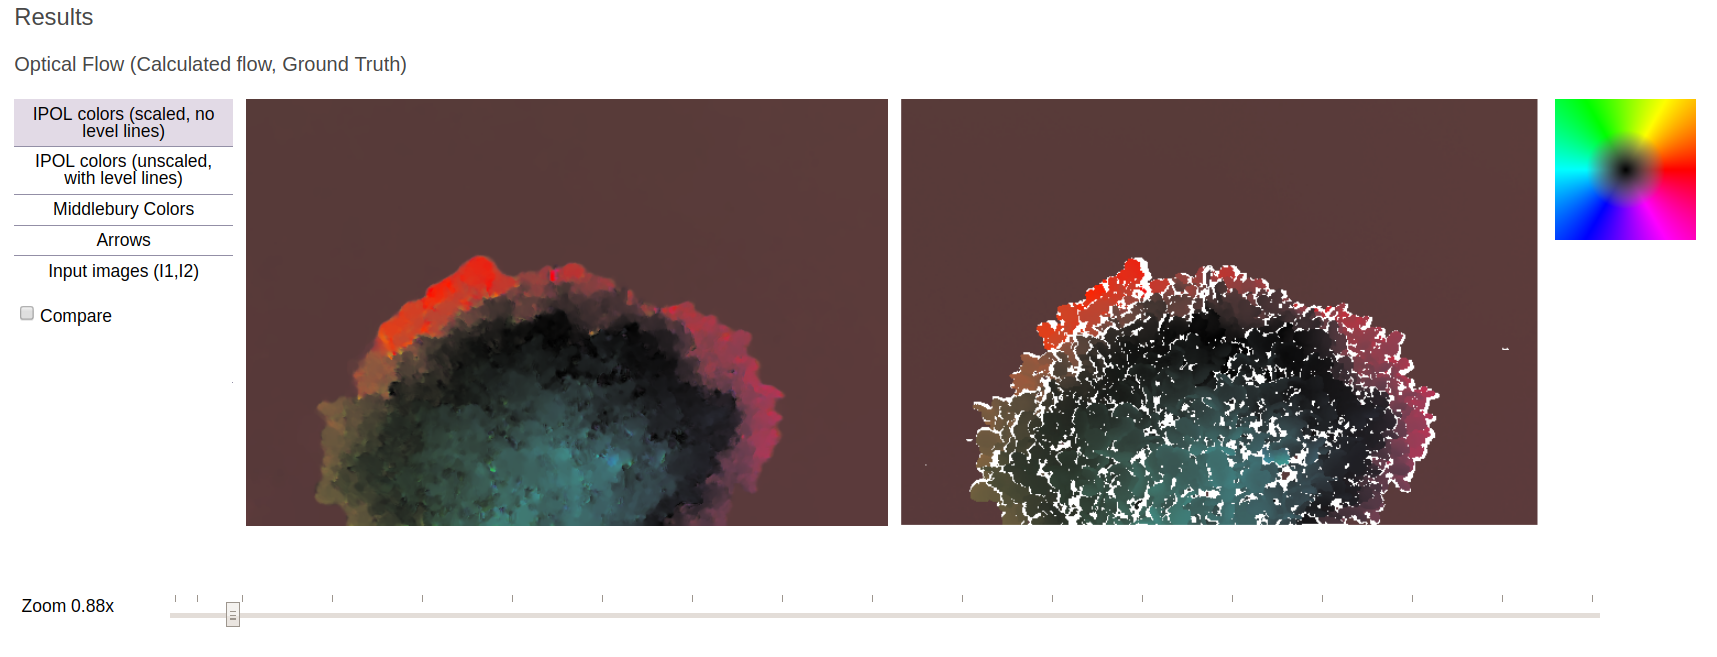
\includegraphics[scale=0.25]{Images/image_gallery_example.png}}
\caption{Example of an image gallery. In this example, we see three images per row.}
\label{fig:image_gallery_example}
\end{figure}

%------ gallery_video  ------
\subsection{The \emph{gallery\_video} type}

The results \emph{gallery\_video} type displays video files. This type is quite similar to the previous one but related to the visualization of video contents.

\begin{longtable}{|>{\bf}L{\dimexpr 0.15\linewidth}|L{\dimexpr 0.7\linewidth}|c|}
\hline
 \centering {key}     & \centering {\bf description} & {\bf req} 
\tabularnewline \hline \hline
 type       & gallery\_video  & yes \\ \hline
 visible    & A Javascript expression evaluated as a boolean. & no \\ \hline
 label      & HTML label for the gallery, can be either a single string or 
             a list of string that will be concatenated. & no \\ \hline
 contents   & A set of sets, each entry describes one or more images with a key and properties:
\vspace{-1em}
\begin{itemize}
    \setlength\itemsep{-0.5em}
    \item \textit{key}, required, a label for the entry, could be a string or an evaluated expression in case of repeat;
    \item \textit{img}, required, a string with a filename or an array of strings with filenames;
    \item \textit{visible}, optional, a Javascript expression evaluated to a boolean;
    \item \textit{repeat}, optional, a Javascript expression, will create a loop in the form idx=0..range-1
\end{itemize} 
\vspace{-1em} & yes \\ \hline
\caption{Properties of the \emph{gallery\_video} type in the results section.}
\end{longtable}

\paragraph{Examples:}
Advanced example, mixing repeat, visible, using an array of filenames.
\begin{lstlisting}[language=json,firstnumber=1]
{
    "type": "video_gallery",
    "label": "<b>Video gallery</b>",
    "display": "grid",
    "visible": "1==1",
    "contents": {
        "Input_0": {
            "video":  "'input_0.mp4'",
            "visible": "1==1"
        },
        "'Scale_'+idx": {
            "video":  "'scaled_'+idx+'.mp4'",
            "repeat": "4"
        }
    }
}
\end{lstlisting}



%------ file_download  ------
\subsection{The \emph{file\_download} type}

The results \emph{file\_download} type proposes a link to download a file.

\begin{longtable}{|>{\bf}L{\dimexpr 0.15\linewidth}|L{\dimexpr 0.7\linewidth}|c|}
\hline
\centering {key}     & \centering {\bf description} & {\bf req} \tabularnewline 
\hline \hline
 type      & file\_download  & yes \\ \hline
 visible    & A Javascript expression evaluated as a boolean. & no \\ \hline
 repeat    & range expression (evaluated in Javascript):
              will create a loop in the form idx=0..range-1 & no \\ \hline
 label     & HTML title associated to the file to download. In case of repeat, 
            evaluated as an expression with idx variable, otherwise, can be evaluated
            if it starts with a single quote.& yes \\ \hline
 contents  & either a single string of the filename to download, or a list
              of label:filename pairs for files to download. In case of repeat, 
            evaluated as an expression with idx variable. & yes \\ \hline
\caption{Properties of the \emph{file\_download} type in the results section.}
\end{longtable}

We show two examples: the first one is to download one result and the second is to download several results in the same line.

\paragraph{Examples}:\\
\begin{lstlisting}[language=json,firstnumber=1]
{ 
    "type"     : "file_download", 
    "label"    : "Download Hough result",
    "contents" : "output_hough.png" 
}
\end{lstlisting}

\begin{lstlisting}[language=json,firstnumber=1]
{
    "type"     : "file_download", 
    "label"    : "<h3>Download computed optical flow:</h3>",
    "contents" : {
        "tiff": "stuff_tvl1.tiff", 
        "flo" : "stuff_tvl1.flo",
        "uv"  : "stuff_tvl1.uv"
    }
}
\end{lstlisting}
Example using \emph{repeat}:
\begin{lstlisting}[language=json,firstnumber=1]
{ 
    "type"     : "file_download", 
    "repeat"   : "params.scales",
    "label"    : "'Download the estimations obtained at scale '+idx",
    "contents" : "'estimation_s'+idx+'.txt'"
}
\end{lstlisting}

%------ html_text  ------
\subsection{ \emph{html\_text} type}

It \emph{html\_text} renders the contents of a file as HTML code.

\begin{longtable}{|>{\bf}L{\dimexpr 0.15\linewidth}|L{\dimexpr 0.7\linewidth}|c|}
\hline
\centering {key}     & \centering {\bf description} & {\bf req} \tabularnewline 
\hline \hline
 type      & html\_text  & yes \\ \hline
 visible    & A Javascript expression evaluated as a boolean. & no \\ \hline
 contents  & An array of strings, that will be concatenated to form the HTML 
             content. This content can contain Javascript expression if it starts
            with a single quote. & yes \\ \hline
\caption{Properties of the \emph{html\_text} type in the results section.}
\end{longtable}

\paragraph{Example}:\\
\begin{lstlisting}[language=json,firstnumber=1]
{ 
    "type"          : "html_text", 
    "contents"      : [
        "'<p style=\"font-size:85%\">",
        "* &ldquo;Exact&rdquo; is computed with FIR, ",
        "DCT for &sigma;&nbsp;&gt;&nbsp;2 ",
        "(using '+params.sigma<=2?'FIR':'DCT'+",
        "'</p>'" 
    ] 
}
\end{lstlisting}


%------------ text_file --------------------------
\subsection{ \emph{text\_file} type}

The results \emph{text\_file} type displays a text file.

\begin{longtable}{|>{\bf}L{\dimexpr 0.15\linewidth}|L{\dimexpr 0.7\linewidth}|c|}
\hline
\centering {key}     & \centering {\bf description} & {\bf req} \tabularnewline 
\hline \hline
 type      & text\_file  & yes \\ \hline
 visible    & Javascript expression evaluated as a boolean. & no \\ \hline
 label     & HTML label. & yes \\ \hline
 contents  & A text filename to display. & yes \\ \hline
 style     & CSS rules written in a JSON string, ex 
             \texttt{"style": "\{'font-weight': 'bolder', 'color': 'red'\}"} & yes \\ \hline
\caption{Properties of the \emph{text\_file} type in the results section.}
\end{longtable}

\paragraph{Example}:\\
\begin{lstlisting}[language=json,firstnumber=1]
{ 
    "type"          : "text_file", 
    "label"         : "<h2>Output<h2>",
    "contents"      : "stdout.txt",
    "style"         : "{'width': '40em', 'height': '16em', 'background-color': '#FFE'}"
}
\end{lstlisting}


%------ message  ------
\subsection{ \emph{message} type}

The \emph{message} type displays a text message with a predefined color. This can be 
used for warning or error messages.

\begin{longtable}{|>{\bf}L{\dimexpr 0.15\linewidth}|L{\dimexpr 0.7\linewidth}|c|}
\hline
 \centering {key}     & \centering {\bf description} & {\bf req} \tabularnewline 
\hline \hline
 type       & message  & yes \\ \hline
 visible    & Javascript expression evaluated as a boolean. & no \\ \hline
 contents   & A string which will be evaluated by Javascript to get the message. & yes \\ \hline
 textColor  & The name of a color or a CSS-compatible color. & no \\ \hline
\caption{Properties of the \emph{message} type in the results section.}
\end{longtable}

\paragraph{Examples}:\\
\begin{lstlisting}[language=json,firstnumber=1]
{    
    "contents": "'Image too small: the input image needs to be at least 42000 pixels to get a reliable estimate<br> Forced to use one bin for the estimation.'", 
    "type": "message", 
    "textColor": "red",
    "visible": "info.sizeX * info.sizeY < 42000" 
}
\end{lstlisting}
